

\section{Motivating Applications}\label{sec:motivation}
\begin{table*}[t]
\begin{center}
    \begin{tabular}{|l|c|c|c|c|}
    \hline
    \multicolumn{1}{|c|}{\bf Application} & 
    \multicolumn{1}{c|}{\bf Existing Solution} & 
    \multicolumn{1}{c|}{\bf Attributes} & 
    \multicolumn{1}{c|}{\bf Tag Field} & 
    \multicolumn{1}{c|}{\bf Tags Conveyed By}\\ \hline
    SDN-enabled IXP & iSDX~\cite{isdx} & Advertising peers & Destination MAC & ARP \\ \hline
    Service chaining & FlowTags~\cite{flowtags} & Middleboxes & IP Fragment Field & First Middlebox \\ \hline
    Policy enforcement & Alpaca~\cite{alpaca} & Host permissions & IP Source Address & DHCP \\ \hline
    \end{tabular}
\end{center}
    \caption{Example applications and systems which have solved them by some form of tagging.} 
    \label{tab:applications}
\end{table*}

There are many applications where encoding and reading FECs is of interest, and in particular we will look at three of them, which are outlined in Table \ref{tab:applications}.
 
\subsection{Software-Defined IXPs}
\begin{figure}[t!] 
\begin{minipage}{1\linewidth}
\begin{subfigure}[b]{0.96\linewidth}
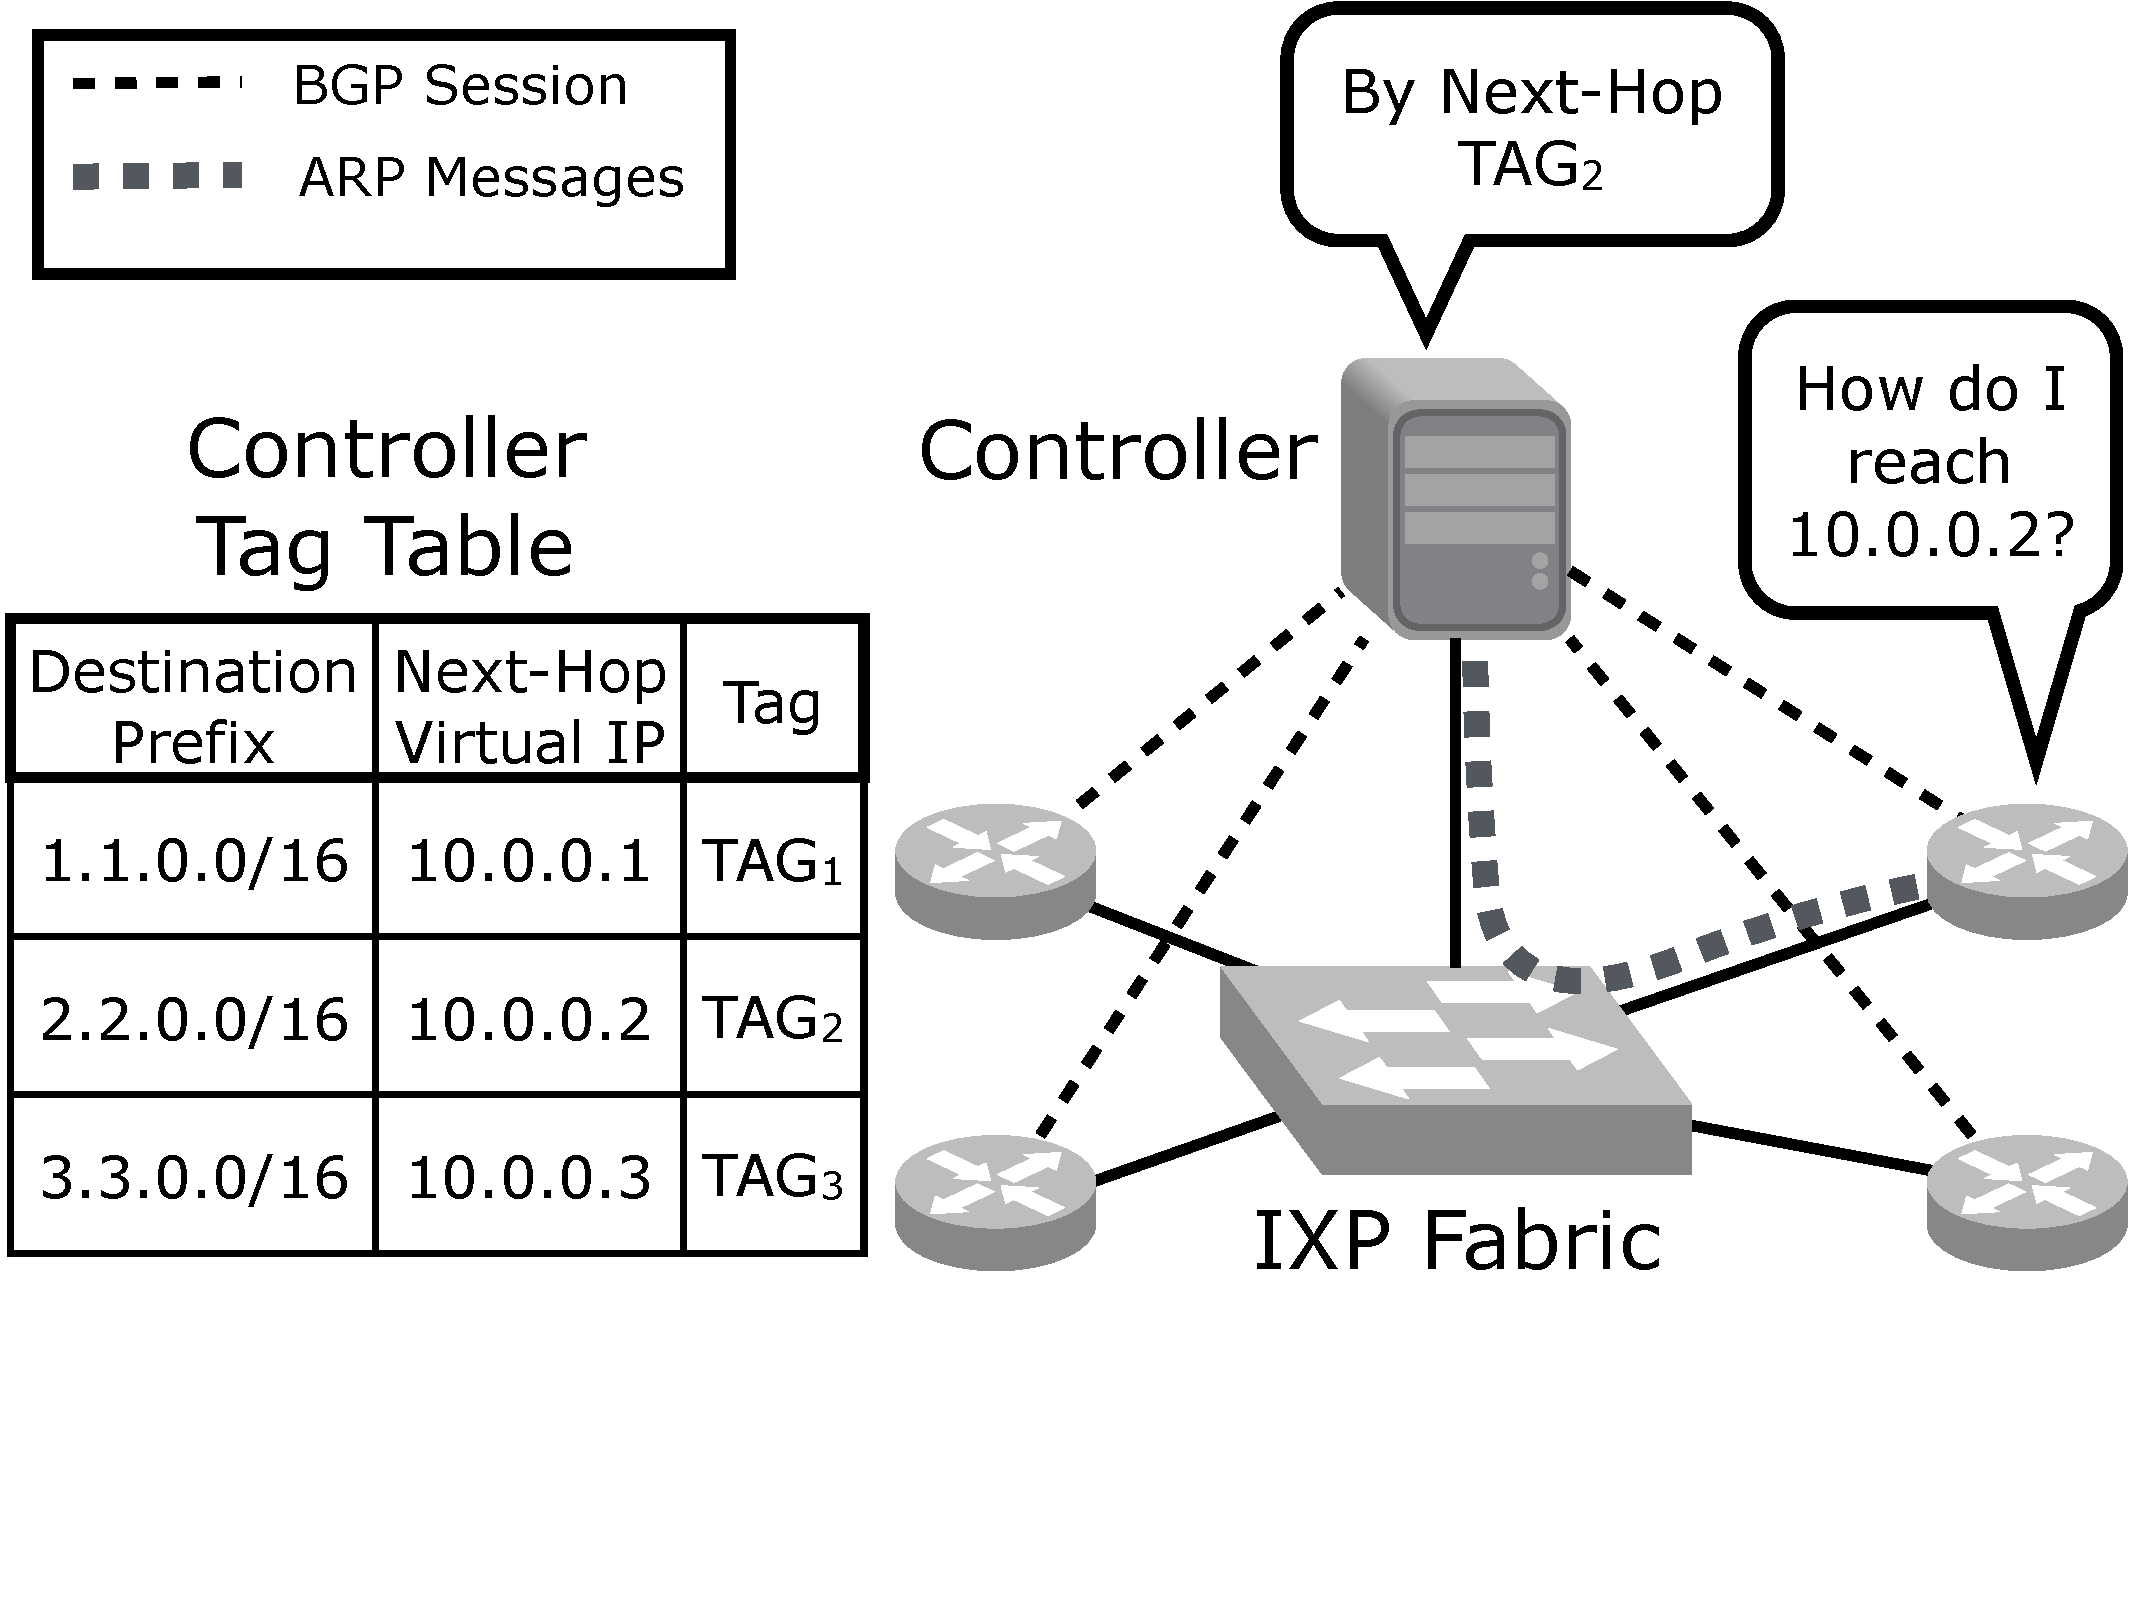
\includegraphics[width=\linewidth,trim={0 5cm 0 0}]{figures/sdx_example}
\end{subfigure} 
\end{minipage} 
\caption{An example of a Software-Defined IXP system, as presented in the iSDX paper~\cite{isdx}. Border routers connect to the IXP fabric and initiate BGP sessions with the controller. Each router announces routes for IP prefixes to the controller, and the controller aggregates these, computes FECs for each IP prefix, and announces a Virtual Next-hop (VNH) IP address for IXP participants to reach that prefix. When a participant attempts to send traffic to a VNH IP, it first sends an ARP request for the MAC of that VNH to the IXP fabric. The controller intercepts this, and responds with a tag as the destination MAC. The participant then forwards packets to the IXP fabric with the appropriate tag in the destination MAC address field.}
\label{fig:sdx_example}
\end{figure}
At an Internet Exchange Point (IXP), multiple autonomous systems (ASes)
connect at a single logical interconnect to exchange traffic and
interdomain routing information.  At an IXP with support for SDN
policies, the connected ASes may wish to enact fine-grained 
policies based on attributed beyond a packet's destination
address. Supposed that $AS_1$ wants to send as much of their HTTP traffic
to $AS_2$ as possible. $AS_2$ may not have routes to every HTTP
destination, so it is incorrect for this AS to receive all HTTP traffic,
regardless of destination. If
the routing policies do not account for the routes of each AS, traffic
may be forwarded to networks that cannot handle it.

The initial SDX design used flat tags to encode these distinct
forwarding decisions~\cite{sdx}, with the architecture shown in Figure \ref{fig:sdx_example}. Each AS shares its list of routes with
a central controller, and every unique set of routes is assigned a flat
tag. The controller then attaches these tags to every packet by
announcing them to all peers as destination MAC addresses via ARP
replies. The fine-grained routing policies are then modified by the
controller to read tags before making a routing decision.  This flat
tagging approach encounters into memory scalability challenges as a
direct result of flat tagging, which were remedied by the followup work
iSDX~\cite{isdx}. iSDX used a precursor to our tagging scheme, taking
advantage of OpenFlow 1.3's support for wildcard matching on destination
MAC addresses.

\subsection{Service Chaining}
Network operators often want network traffic to be directed through a
sequence of middleboxes, such as load balancers or firewalls.  Different
flows may be subject to different chains of middleboxes, and it can be a
challenge to design the network in such a way that every flow traverses
only the needed set of middleboxes. Additionally, middleboxes may modify
packet headers, obscuring the original source of the flow and making it
unclear which middlebox chain should be followed.
FlowTags~\cite{flowtags} uses tags to encode how each middlebox should
process each packet. To compress policy information into small,
repurposed header fields, FlowTags uses flat tags, where each tag maps
to a middlebox sequence and the packet's origin host. Whenever a
middlebox sees a new flow, it communicates with a central controller to
establish a new tag.  Yet, FlowTags does not evaluate the number of
forwarding table entries that such a flat tagging scheme might
require. Because many flows may be forwarded through similar sequences
of middleboxes, we expect that service chaining may benefit from the
attribute-based tagging approach we present in this work.
 

\subsection{Host Attributes for Network Policies}
In some situations, network policies depend on the traffic sender.  For
example, users in departments within an organization may be subject
to different quality of service or access control policies. If
department information is not attached to packets directly, it must be
inferred from some combination of packet header fields, which can result
in unnecessarily complex forwarding tables.  Alpaca~\cite{alpaca}
encodes policy information in IP addresses and assigns these addresses
to network hosts via DHCP. Although not explicitly a tag, these IP
addresses can be thought of as a tag appended to the network's IP
prefix. Alpaca takes advantage of prefix and wildcard matching when
constructing tags to circumvent the memory scalability challenges of
index tagging, yet each host must receive a different tag, because each
IP must be unique. FEC-based tagging could provide significant
opportunities for aggregation in this setting.


%\paragraph{Multicast and Anycast}
%In a classic IP anycast scenario, a single service is replicated across multiple servers to attempt to lighten the maximum load that any single server receives. Since each server hosts the same server, they can all equivalently handle packets destined for that service. Each server is assigned the same IP address, and the network forwards any traffic destined for the shared IP address to the nearest replica of the service. However, if each server has a set of services it replicates, but sets differ across servers, no two servers can be treated equally and receive identical IP addresses. If lists of servers could be attached to packet headers, the network could read this list and choose a server to handle the packet. 
%The scenario of Multicast is similar, where a list of subscribers can be attached to the packet header of a multicast packet. The network would then read this list and replicate the packet towards each subscriber. 